%%%%%%%%%%%%%%%%%%%%%%%%%%%%%%%%%%%%%%%%%%%%%%%%%%%
%
%  New template code for TAMU Theses and Dissertations starting Fall 2016.
%
%
%  Original Author: Sean Zachary Roberson
%  This version adapted for URS by Parasol lab.
%  Adapted from version 3.16.10, which was last updated on 9/29/2016.
%  URS adaptation last updated 1/9/2017.
%\part{title}
%%%%%%%%%%%%%%%%%%%%%%%%%%%%%%%%%%%%%%%%%%%%%%%%%%%

\documentclass[12pt]{report}

%These next lines change the font. Fixes for certain
%fonts will be implemented in a future release.

%Comment this line if you do not wish to use Times
%New Roman. The font used will then be the LaTeX
%default of Computer Modern.
\usepackage{times}
%\usepackage{cmbright}
\usepackage[T1]{fontenc}

%Do not change these settings. The geometry package
%Adjusts the margins to those specified by the Thesis
%Manual.
\usepackage[letterpaper]{geometry}
\geometry{verbose,tmargin=1.25in,bmargin=1.25in,lmargin=1.4in,rmargin=1.15in}
\usepackage[doublespacing]{setspace}
\usepackage{packages/tocloft}
\usepackage[rm, tiny, center, compact]{packages/titlesec}
\usepackage{indentfirst}
\usepackage{etoolbox}

\usepackage{packages/tocvsec2}
\usepackage[titletoc]{packages/appendix}
\usepackage{packages/appendix}
\usepackage{tamuconfig}

\usepackage{rotating}

%These are common AMS packages. Many LaTeX documents
%have these packages declared in their preambles.
\usepackage{amsmath, amsthm}

%This package allows for the use of graphics in the
%document.
\usepackage{graphicx}

%It is best practice to keep all your pictures in
%one folder inside the main directory in which your
%TeX file is kept. Here the folder is named "graphic."
%Replace the name here with your folder's name, if needed.
%The period is needed due to relative referencing.
\graphicspath{ {./graphic/} }

%If needed, this will allow you to add the word "Page"
%to extra pages on your front matter lists.
\usepackage{afterpage}

%This is from the mdwtools package; it fixes some
%footnote commands and allows you to have footnotes in
%tables via the savenotes environment.
\usepackage{footnote}
\usepackage{chngcntr}
\counterwithout{footnote}{chapter}


% Added to fix issues with pdf searching in some versions of LaTeX
%\usepackage[T1]{fontenc}\usepackage{lmodern}
%%%%%%%%%%%%%%%%%%%%%%%%%%%%%

% Hyperref setup below.  You should be able to get away with using uncommenting just the first line.
%\usepackage[hidelinks]{hyperref}

% if \usepackage[hidelinks]{hyperref} doesn't work try this.
%\usepackage{hyperref}  % Hidelinks is an option that removes link visiability.  TAMU Thesis Offices prefers to not see the links. But often doesn't work.
%
%\hypersetup{
%    colorlinks=true,
%    linkcolor=black,
%    citecolor=black,
%    filecolor=black,
%    urlcolor=black,
%}
%%%%%%%  End of hyperref setup.  One of these two options should work, but my motto with hyperref is when in doubt, comment it out!
%%%%%%%%%  This hopefully fixes the problem with vertical spacing of section headings at the top of the page..  Commented out in 1.0.7
% \preto\section{%
% \ifnum\value{section}>0\addtocontents{toc}{\vskip-6pt}\fi
% }
% \preto\subsection{%
% \ifnum\value{subsection}=0\addtocontents{toc}{\vskip-6pt}\fi
% \ifnum\value{subsection}>0\addtocontents{toc}{\vskip-6pt}\fi
% }
%%%%%%%%%%%%%%%%%%%%%%%%%%%%%%%%%%%%%%%%%%%%%%%%%%%%%%

\begin{document}

%The title of your document goes here.
%Spacing may need to be adjusted if your title is long
%and pushes the copyright off the page.
\renewcommand{\title}{textbook problem dependency web}

\newcommand{\abstracttitle}{Textbook Problem Dependency Web}

\renewcommand{\author}{Joseph Martinsen}

%Your department name goes here.
\newcommand{\department}{Computer Engineering}

\newcommand{\program}{Undergraduate Research Scholar}

\newcommand{\ursadvisor}{Philip B. Yasskin}
\newcommand{\advisordepartment}{Mathematics}

% Doesn't change until next year.
\newcommand{\ursmonth}{May}
\newcommand{\ursyear}{2018}

%\titleformat{\chapter}[display]
%{\normalfont\bfseries\filcenter}{\chaptertitlename\
%\thechapter}{14pt}{\fontsize{14pt}{12pt}}

%%%%%%%%%%%%%%%%%%%%%%%%%%%%%%%%%%%%%%%%%%%%%%%%%%%
%
%  New template code for TAMU Theses and Dissertations starting Fall 2016.
%
%
%  Original Author: Sean Zachary Roberson
%  This version adapted for URS by Parasol lab.
%  Adapted from version 3.16.10, which was last updated on 9/29/2016.
%  URS adaptation last updated 1/9/2017.
%
%%%%%%%%%%%%%%%%%%%%%%%%%%%%%%%%%%%%%%%%%%%%%%%%%%%

%%%%%%%%%%%%%%%%%%%%%%%%%%%%%%
%% TITLE PAGE
%% The values get updated automatically.  Please do not make changes to this file other than adding/deleting committee members where necessary.
%%%%%%%%%%%%%%%%%%%%%%%%%%%%%%

\providecommand{\tabularnewline}{\\}



\begin{titlepage}

\begin{center}
\MakeUppercase{\textbf{\large{\title}}}
\vspace{4em}

An Undergraduate Research Scholars Thesis

by

\MakeUppercase{\author}

\vspace{4em}

\begin{singlespace}

Submitted to the Undergraduate Research Scholars program at\\
Texas A\&M University \\

in partial fulfillment of the requirements for the designation as an\\

\end{singlespace}

\vspace{2em}
\MakeUppercase{\program}
\par\end{center}

\begin{singlespace}
  \begin{tabular}{ll}
    & \tabularnewline & \cr
  \end{tabular}
\end{singlespace}

\begin{center}
  \vspace{\baselineskip}
  \begin{singlespace}
    Approved by Research Advisor:\hfill~Dr.~\ursadvisor
  \end{singlespace}
  \vspace{\baselineskip}
\end{center}


\begin{center}
\ursmonth \hspace{2pt} \ursyear

\vspace{3em}

Major: \department \par

\vspace{3em}

\par\end{center}
\end{titlepage}
\pagebreak{}




 % This is simply a file that formats and adds your titlepage, please do not edit this unless you have a specific need. .

%%%%%%%%%%%%%%%%%%%%%%%%%%%%%%%%%%%%%%%%%%%%%%%%%%%
%
%  New template code for TAMU Theses and Dissertations starting Fall 2016.
%
%
%  Original Author: Sean Zachary Roberson
%  This version adapted for URS by Parasol lab.
%  Adapted from version 3.16.10, which was last updated on 9/29/2016.
%  URS adaptation last updated 1/9/2017.
%
%%%%%%%%%%%%%%%%%%%%%%%%%%%%%%%%%%%%%%%%%%%%%%%%%%%
%%%%%%%%%%%%%%%%%%%%%%%%%%%%%%%%%%%%%%%%%%%%%%%%%%%%%%%%%%%%%%%%%%%%%%
%%       TABLE OF CONTENTS
%%%%%%%%%%%%%%%%%%%%%%%%%%%%%%%%%%%%%%%%%%%%%%%%%%%%%%%%%%%%%%%%%%%%%
% single-space sections in Table of Contents  - commented in version 1.7
%\renewcommand{\cftsecafterpnum}{\vskip0.5\baselineskip}
%\renewcommand{\cftsubsecafterpnum}{\vskip0.5\baselineskip}
%\renewcommand{\cftsubsubsecafterpnum}{\vskip0.5\baselineskip}
%%%%%%%%%%%%%%%%%%%%%%%%%%%%%%%%%%%%%%%%%%%%%%%%%%%

\phantomsection
\pagenumbering{gobble}
%\addcontentsline{toc}{chapter}{TABLE OF CONTENTS}

\begin{singlespace}
  \renewcommand\contentsname{\normalfont}
  {\centerline{{\textbf{\large{TABLE OF CONTENTS}}}}}

%\setcounter{tocdepth}{4} % This puts \subsubsection[]{×} in your List of Tables.  The default is 3.

\setcounter{tocdepth}{1}

%%%%%%%%%%%%%  Adds Page above the page number in TOC
\setlength{\cftaftertoctitleskip}{1em}
\renewcommand{\cftaftertoctitle}{%
\hfill{\normalfont {Page}\par}}


\tableofcontents

%\addtocontents{toc}{\protect\afterpage{~\hfill\normalfont{Page}\par\medskip}}
\end{singlespace}

\pagebreak{}
  % This adds the table of contents, please do not edit this unless you have a specific need.
%%%%%%%%%%%%%%%%%%%%%%%%%%%%%%%%%%%%%%%%%%%%%%%%%%%
%
%  New template code for TAMU Theses and Dissertations starting Fall 2016.
%
%
%  Original Author: Sean Zachary Roberson
%  This version adapted for URS by Parasol lab.
%  Adapted from version 3.16.10, which was last updated on 9/29/2016.
%  URS adaptation last updated 1/9/2017.
%
%%%%%%%%%%%%%%%%%%%%%%%%%%%%%%%%%%%%%%%%%%%%%%%%%%%
%%%%%%%%%%%%%%%%%%%%%%%%%%%%%%%%%%%%%%%%%%%%%%%%%%%%%%%%%%%%%%%%%%%%%
%%                           ABSTRACT
%%%%%%%%%%%%%%%%%%%%%%%%%%%%%%%%%%%%%%%%%%%%%%%%%%%%%%%%%%%%%%%%%%%%%

\chapter*{ABSTRACT}

\addcontentsline{toc}{chapter}{ABSTRACT} % Needs to be set to part, so the TOC doesnt add 'CHAPTER ' prefix in the TOC.

\pagestyle{plain} % No headers, just page numbers
\pagenumbering{arabic} % Arabic numerals
\setcounter{page}{1}
\begin{center}

\begin{singlespace}
\abstracttitle
\end{singlespace}
\vspace{2em}
\begin{singlespace}
\author \\
Department of \department \\
Texas A\&M University \\
\end{singlespace}
\vspace{2em}
\begin{singlespace}
Research Advisor: Dr. \ursadvisor \\
Department of \advisordepartment \\
Texas A\&M University \\
\end{singlespace}
\end{center}
\vspace{2em}

\indent This is the first numbered page Arabic numeral 1. Page
numbers are outside the 1 inch margins (on all sides), at the bottom of the page and centered; everything else is inside the margins. No bold on this page (Exception: heading ABSTRACT is bold if major headings are bold. Text begins two double spaces below the major heading. Recommended length of
text is no more than 350 words. Vertical spacing is double spaced or
space-and-a-half. (\emph{This \LaTeX ~ template applies double space for this
ABSTRACT.}) The same margin settings and text alignment are followed else where
in this thesis. There should be no numbered references or formal citations in
the ABSTRACT.

The content of this ABSTRACT provides a complete, succinct snapshot of the
research, addressing the purpose, methods, results, and conclusions of the
research. As a result, it should stand alone without any formal citations or
references to chapters/sections of the work. To accommodate with a variety of online database, images or complex equations should also be avoided.

The next pages are Dedication, Acknowledgments, and Nomenclature.


\pagebreak{}

%%%%%%%%%%%%%%%%%%%%%%%%%%%%%%%%%%%%%%%%%%%%%%%%%%%
%
%  New template code for TAMU Theses and Dissertations starting Fall 2016.
%
%
%  Original Author: Sean Zachary Roberson
%  This version adapted for URS by Parasol lab.
%  Adapted from version 3.16.10, which was last updated on 9/29/2016.
%  URS adaptation last updated 1/9/2017.
%
%%%%%%%%%%%%%%%%%%%%%%%%%%%%%%%%%%%%%%%%%%%%%%%%%%%
%%%%%%%%%%%%%%%%%%%%%%%%%%%%%%%%%%%%%%%%%%%%%%%%%%%%%%%%%%%%%%%%%%%%%%
%%                           DEDICATION
%%%%%%%%%%%%%%%%%%%%%%%%%%%%%%%%%%%%%%%%%%%%%%%%%%%%%%%%%%%%%%%%%%%%%
\chapter*{DEDICATION}
\addcontentsline{toc}{chapter}{DEDICATION}


\begin{center}
\vspace*{\fill}
To my everything, Savannah.
\vspace*{\fill}
\end{center}

\pagebreak{}

%%%%%%%%%%%%%%%%%%%%%%%%%%%%%%%%%%%%%%%%%%%%%%%%%%%
%
%  New template code for TAMU Theses and Dissertations starting Fall 2016.
%
%
%  Original Author: Sean Zachary Roberson
%  This version adapted for URS by Parasol lab.
%  Adapted from version 3.16.10, which was last updated on 9/29/2016.
%  URS adaptation last updated 1/9/2017.
%
%%%%%%%%%%%%%%%%%%%%%%%%%%%%%%%%%%%%%%%%%%%%%%%%%%%


%%%%%%%%%%%%%%%%%%%%%%%%%%%%%%%%%%%%%%%%%%%%%%%%%%%%%%%%%%%%%%%%%%%%%%
%%                           ACKNOWLEDGMENTS
%%%%%%%%%%%%%%%%%%%%%%%%%%%%%%%%%%%%%%%%%%%%%%%%%%%%%%%%%%%%%%%%%%%%%
\chapter*{ACKNOWLEDGMENTS}
\addcontentsline{toc}{chapter}{ACKNOWLEDGMENTS}  % Needs to be set to part, so the TOC doesnt add 'CHAPTER ' prefix in the TOC.


\indent This section is also optional, limited to four pages. It must follow the Dedication Page (or Abstract, if no Dedication). If listing preliminary pages in Table of Contents, include Acknowledgments. Heading (\MakeUppercase{Acknowledgments}) is bold if major headings are bold. It should be in same type size and style as text. So does vertical spacing, paragraph style, and margins. Also, ensure that the spelling of ``acknowledgments'' matches throughout the text and the table of contents.

\pagebreak{}

%%%%%%%%%%%%%%%%%%%%%%%%%%%%%%%%%%%%%%%%%%%%%%%%%%%
%
%  New template code for TAMU Theses and Dissertations starting Fall 2016.
%
%
%  Original Author: Sean Zachary Roberson
%  This version adapted for URS by Parasol lab.
%  Adapted from version 3.16.10, which was last updated on 9/29/2016.
%  URS adaptation last updated 1/9/2017.
%
%%%%%%%%%%%%%%%%%%%%%%%%%%%%%%%%%%%%%%%%%%%%%%%%%%%

%%%%%%%%%%%%%%%%%%%%%%%%%%%%%%%%%%%%%%%%%%%%%%%%%%%%%%%%%%%%%%%%%%%%%%
%%                           NOMENCLATURE
%%%%%%%%%%%%%%%%%%%%%%%%%%%%%%%%%%%%%%%%%%%%%%%%%%%%%%%%%%%%%%%%%%%%%

\chapter*{NOMENCLATURE}
\addcontentsline{toc}{chapter}{NOMENCLATURE}  % Needs to be set to part, so the TOC doesnt add 'CHAPTER ' prefix in the TOC.

%A note about aligning: These entries will align
%themselves according to the ampersand (&).
%No extra spaces are needed, as seen in some of
%the entries below.
\vspace{-0.5in}
	\begin{table}[htbp]
	    \begin{tabular}{@{}p{0.33\textwidth} p{0.62\textwidth}@{}}
		Editor & A particular instructor, representative of the adopting institution or publisher who wants to reorder the textbook\\	[2ex]
		DAG & Directed Acyclic Graph \\ [2ex]
		Net & Refers to the DAG structe use for dependencies \\ [2ex]
		Topic & The content contained in a unit \\ [2ex]
		Unit & Book/Part/Chapter/Section//Cul-de-sac/Page providing the content of the book \\ [2ex]
		Assessment & A tutorial/exercises providing a problem that is given to a student to solve \\ [2ex]
		GUI & Graphical user interface \\ [2ex]
		Graph Database & A particular database utilizes a graph structures for queries with nodes, edges and properties to represent and store data \\ [2ex]
	    \end{tabular}
	\end{table}

\pagebreak{}

%%%%%%%%%%%%%%%%%%%%%%%%%%%%%%%%%%%%%%%%%%%%%%%%%%%
%
%  New template code for TAMU Theses and Dissertations starting Fall 2016.
%
%
%  Original Author: Sean Zachary Roberson
%  This version adapted for URS by Parasol lab.
%  Adapted from version 3.16.10, which was last updated on 9/29/2016.
%  URS adaptation last updated 1/9/2017.
%
%%%%%%%%%%%%%%%%%%%%%%%%%%%%%%%%%%%%%%%%%%%%%%%%%%%
%%%%%%%%%%%%%%%%%%%%%%%%%%%%%%%%%%%%%%%%%%%%%%%%%%%%%%%%%%%%%%%%%%%%%%
%%                           LIST OF FIGURES
%%%%%%%%%%%%%%%%%%%%%%%%%%%%%%%%%%%%%%%%%%%%%%%%%%%%%%%%%%%%%%%%%%%%%

\phantomsection
\addcontentsline{toc}{chapter}{LIST OF FIGURES}

\renewcommand{\cftloftitlefont}{\center\bf\large\MakeUppercase}

\setlength{\cftbeforeloftitleskip}{-12pt} %% Positions the LOF title vertically to match the chapter titles
\renewcommand{\cftafterloftitleskip}{12pt}


\renewcommand{\cftafterloftitle}{%
\\[4em]\mbox{}\hspace{2pt}FIGURE\hfill{\normalfont Page}\vskip\baselineskip}

\begingroup


\begin{center}
\begin{singlespace}
%% These values make the lof table entries appear double spaced between.
\setlength{\cftbeforechapskip}{0.4cm}
\setlength{\cftbeforesecskip}{0.30cm}
\setlength{\cftbeforesubsecskip}{0.30cm}
\setlength{\cftbeforefigskip}{0.4cm}
\setlength{\cftbeforetabskip}{0.4cm}

\listoffigures

\end{singlespace}
\end{center}

\pagebreak{}
  % This adds the list of figures, this is optional. To remove, add a comment '%' at the beggining of the line.
%%%%%%%%%%%%%%%%%%%%%%%%%%%%%%%%%%%%%%%%%%%%%%%%%%%
%
%  New template code for TAMU Theses and Dissertations starting Fall 2016.
%
%
%  Original Author: Sean Zachary Roberson
%  This version adapted for URS by Parasol lab.
%  Adapted from version 3.16.10, which was last updated on 9/29/2016.
%  URS adaptation last updated 1/9/2017.
%
%%%%%%%%%%%%%%%%%%%%%%%%%%%%%%%%%%%%%%%%%%%%%%%%%%%
%%%%%%%%%%%%%%%%%%%%%%%%%%%%%%%%%%%%%%%%%%%%%%%%%%%%%%%%%%%%%%%%%%%%%%
%%                           lIST OF TABLES
%%%%%%%%%%%%%%%%%%%%%%%%%%%%%%%%%%%%%%%%%%%%%%%%%%%%%%%%%%%%%%%%%%%%%%
%
\phantomsection
\addcontentsline{toc}{chapter}{LIST OF TABLES}

\renewcommand{\cftlottitlefont}{\center\bf\large\MakeUppercase}

\setlength{\cftbeforelottitleskip}{-12pt} %% Positions the LOT title vertically to match the chapter titles

%Note that the similar parameter in the LOF is 12pt; this
%is intentional to make the spacing between the headers
%and the first entry look consistent.
\renewcommand{\cftafterlottitleskip}{1pt}


\renewcommand{\cftafterlottitle}{%
\\[4em]\mbox{}\hspace{2pt}TABLE\hfill{\normalfont Page}\vskip\baselineskip}

\begin{center}
\begin{singlespace}

%% These values make the lot table entries appear double spaced between.
\setlength{\cftbeforechapskip}{0.4cm}
\setlength{\cftbeforesecskip}{0.30cm}
\setlength{\cftbeforesubsecskip}{0.30cm}
\setlength{\cftbeforefigskip}{0.4cm}
\setlength{\cftbeforetabskip}{0.4cm}

\listoftables

\end{singlespace}
\end{center}
\endgroup
\pagebreak{}  % Need this for the pagenumbering to be correct.
  % This adds the list of tables, this is optional. To remove, add a comment '%' at the beginning of the line.

%%%%%%%%%%%%%%%%%%%%%%%%%%%%%%%%%%%%%%%%%%%%%%%%%%%
%
%  New template code for TAMU Theses and Dissertations starting Fall 2016.
%
%
%  Original Author: Sean Zachary Roberson
%  This version adapted for URS by Parasol lab.
%  Adapted from version 3.16.10, which was last updated on 9/29/2016.
%  URS adaptation last updated 1/9/2017.
%
%%%%%%%%%%%%%%%%%%%%%%%%%%%%%%%%%%%%%%%%%%%%%%%%%%%
%%%%%%%%%%%%%%%%%%%%%%%%%%%%%%%%%%%%%%%%%%%%%%%%%%%%%%%%%%%%%%%%%%%%%%
%%                           INTRODUCTION
%%%%%%%%%%%%%%%%%%%%%%%%%%%%%%%%%%%%%%%%%%%%%%%%%%%%%%%%%%%%%%%%%%%%%


\pagestyle{plain} % No headers, just page numbers
%\pagenumbering{arabic} % Arabic numerals
%\setcounter{page}{1}

\chapter{INTRODUCTION}

\section{Background}

Textbooks go through a long and arduous process before a student or professor is able to view and use it. This process requires much work and effort into not only validating the content of the textbook but also validating the ordering of the textbook as whole. Much like a jigsaw puzzle, each chapter fits one after another based on the dependency of the topics being taught. On top of these chapters being ordered, the exercises must also be placed in the correct place in order to not give an exercise that is based on a topic that has not been presented to the reader previously.

After all this work on ordering has been completed (among other meticulous things), the textbook is finally ready for publication. As with many good textbooks, many professors and institutions may enjoy the content within the textbook but would prefer delivering the content to a student in a different order than the current order of the textbook. Most of the time, the work and effort that has gone into meticulously ordering the chapters and exercises must now be revisited again and modified. This process is nearly as time consuming and laborious as the first going through this process and is frequently done imperfectly.

\section{Resulting Platform}

In order to achieve, a full stack web application was built. The integration points from the textbook to the application consists of five networks. In the current version of the platform three of the networks into the platform is all that is required for the structures and dependencies of any given textbook to be fully understood and used.

\begin{figure}[ht]
    \centering
    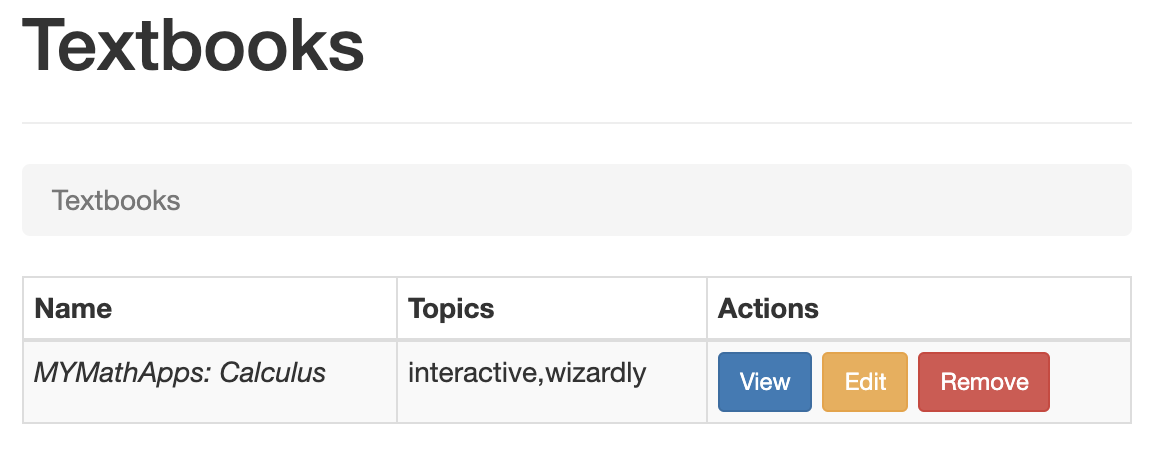
\includegraphics[scale=0.5]{textbooks.png}
    \caption[Textbook selection.]{The selection and upload of networks for a given textbook}
        
    \label{fig:textbooks}
\end{figure}

The next piece of the platform is the most important. It the actual piece of the platform that allows a consumer to reorder and restructure the original ordering of the textbook. It is fully interactive and draggable. Each unit and sub unit can be toggled to view more or less about units. There is also a button to toggle all units to be viewed or to collapse all units until only the independent root units are viewable.

\begin{figure}[ht]
    \centering
    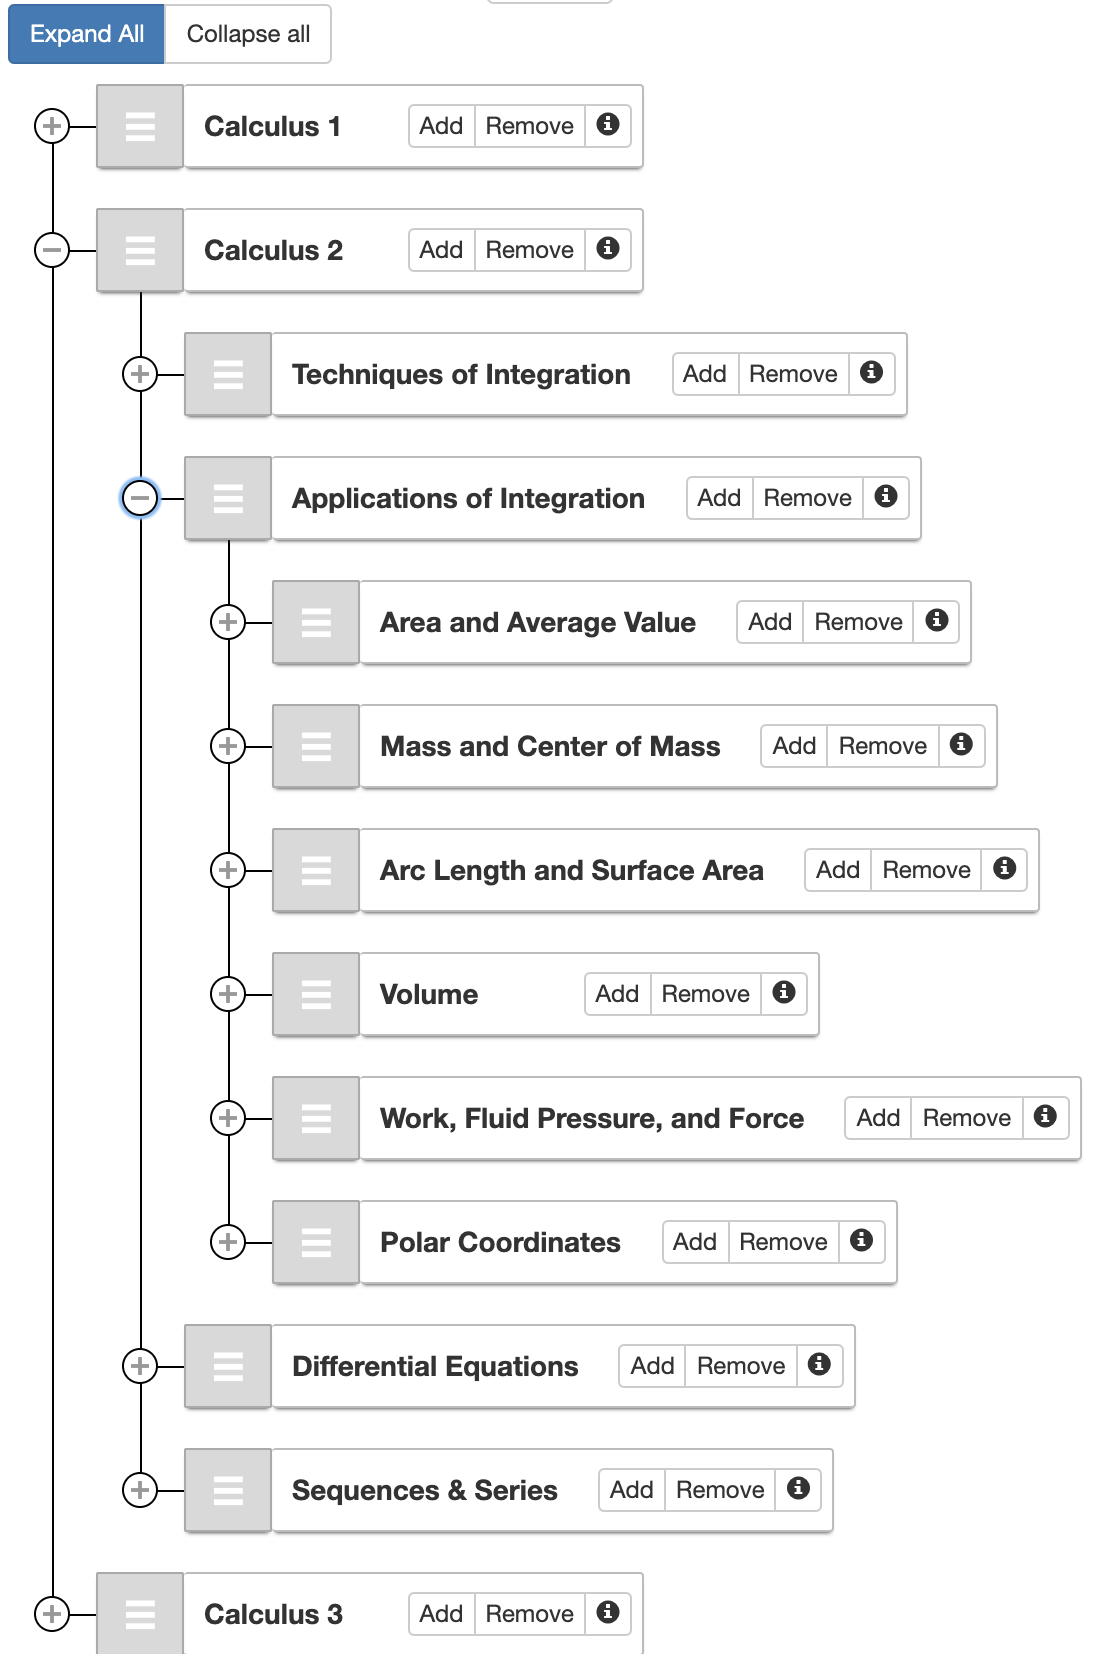
\includegraphics[scale=0.3]{nestedChapters.png}
    \caption[Unit hierarchy.]{Unit hierarchy.}
        
    \label{fig:nestedChapters}
\end{figure}

\pagebreak

On top of being toggleable, each unit is draggable Fig \ref{fig:chaptersMoving}. This allows for each unit to be moved to any other point in the structure of the tree or table of contents. During each of these movements, a request is sent to the server to check the and verify that all dependencies are met. If any dependency is not met, a message is then sent to the front end for it to be displayed to the user.

\begin{figure}[ht]
    \centering
    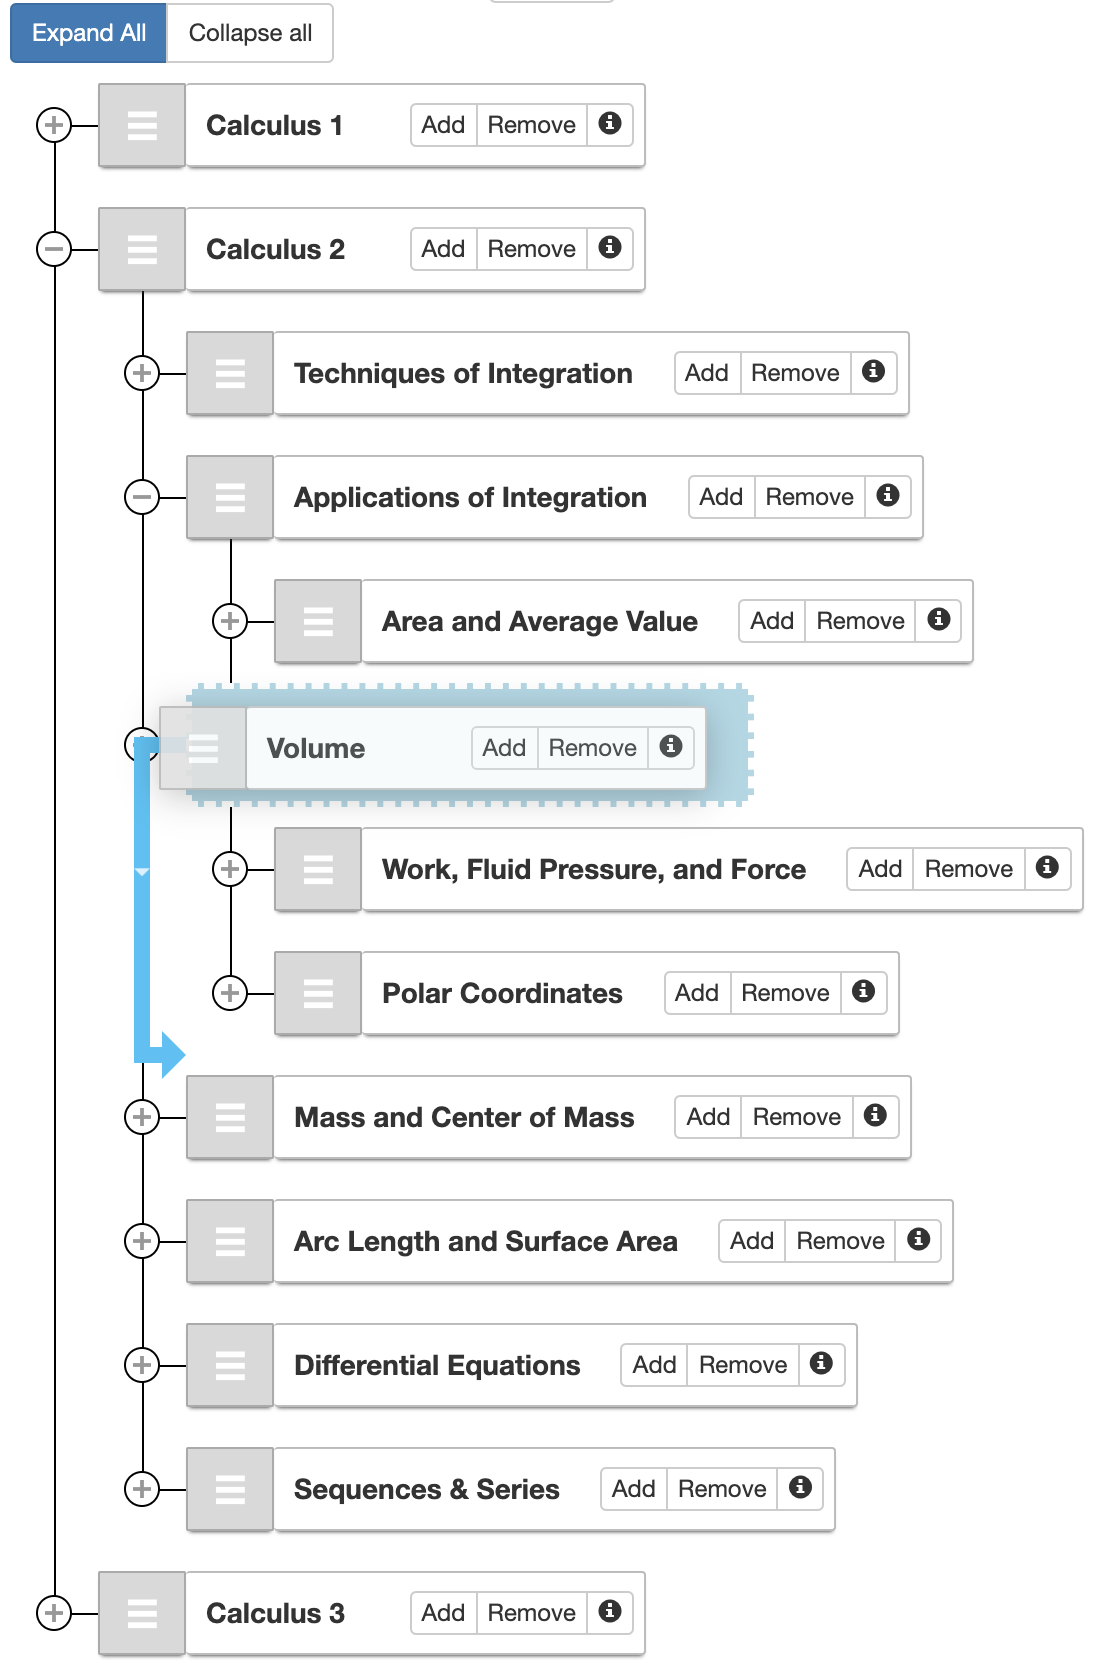
\includegraphics[scale=0.3]{chaptersMoving.png}
    \caption[Reordering units.]{Reordering of units through the use of dragging.}
        
    \label{fig:chaptersMoving}
\end{figure}

\pagebreak

%%%%%%%%%%%%%%%%%%%%%%%%%%%%%%%%%%%%%%%%%%%%%%%%%%%
%
%  New template code for TAMU Theses and Dissertations starting Fall 2016.
%
%
%  Original Author: Sean Zachary Roberson
%  This version adapted for URS by Parasol lab.
%  Adapted from version 3.16.10, which was last updated on 9/29/2016.
%  URS adaptation last updated 1/9/2017.
%
%%%%%%%%%%%%%%%%%%%%%%%%%%%%%%%%%%%%%%%%%%%%%%%%%%%
%%%%%%%%%%%%%%%%%%%%%%%%%%%%%%%%%%%%%%%%%%%%%%%%%%%%%%%%%%%%%%%%%%%%%%%
%%%                           SECTION II
%%%%%%%%%%%%%%%%%%%%%%%%%%%%%%%%%%%%%%%%%%%%%%%%%%%%%%%%%%%%%%%%%%%%%%


\chapter{THE ALGORITHM}

\section{The Design}

\section{The }
% \section{Figures: Placement, Size, and Captions}
% This is a figure template.
% \begin{figure}[ht]
% \centering
% 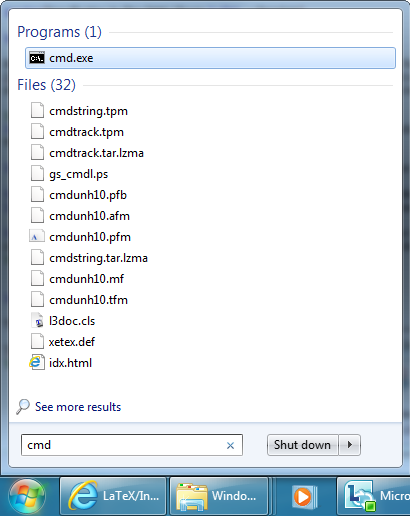
\includegraphics[scale=0.75]{TAMUthesis_CMD_windows.png}
% \caption[The command line compiler in Windows.]{The command line compiler in Windows. It is not suggested that you compile using this method. See compilation instructions in the README.}

% \label{fig:CMD_1}

% \end{figure}

% Figure (and table) titles should be consistent through the document. All
% captions should be placed either above or below the object it describes. This is
% done by placing the \textit{caption} in the correct place. While continued
% figures are allowed by the URS Thesis Manual with proper continuation headings, it is not suggested that any continued figures be included in a \LaTeX\ document.

% The figure below is taken from R. While there are packages available to import
% graphics from R, MATLAB, and similar software, it is probably best to export
% plots generated by these programs as a PNG file, and then import it via the
% \textit{includegraphics} command. Figures must also be referenced in the body
% text within 1 page of where the figure actually appears in the document.

% \begin{figure}[ht]
% 	\centering
% 	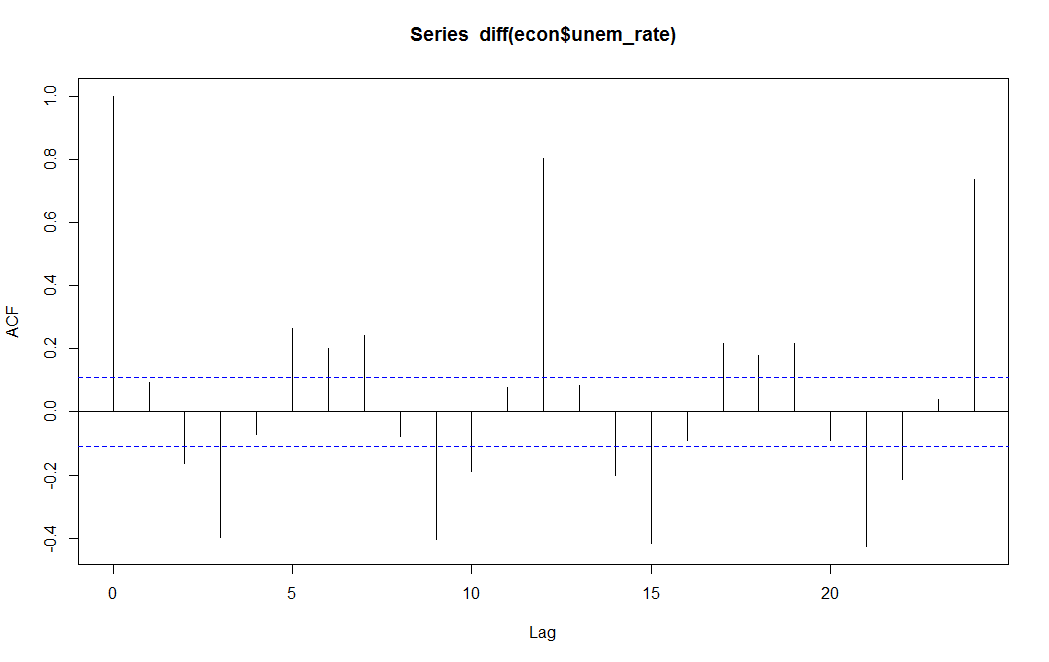
\includegraphics[scale=0.55]{UnemDiffACF.png}
% 	\caption{The autocorrelation function (ACF) of the differenced unemployment series. Seasonal adjustments may be needed.}
% \end{figure}

% \section{Table Placement, Size and Table Title}

% Here is a table, displaying band and auxiliary scores from the 2011 Arcadia Festival of Bands held in Arcadia, CA \cite{ARCADIA}.

% \begin{table}[h!]
% 	\centering

% 	\label{Band}
% 	\caption{Scores from the 2011 Arcadia Festival of Bands.}
%         \vspace{1em}
% 	\begin{tabular}{|l|l|l|}
% 		\hline
% 		School Name & Band Score & Auxiliary Score \\ \hline
% 		Rancho Bernardo & 96.15 & 89.15 \\ \hline
% 		Mt. Carmel & 95.30 & 83.55 \\ \hline
% 		Riverside King & 93.85 & 91.75 \\ \hline
% 		Diamond Bar & 93.20 & 88.60 \\ \hline
% 		El Dorado & 92.80 & 95.45 \\ \hline
% 		Chino & 92.65 & 91.45 \\ \hline
% 		Henry J. Kaiser & 92.60 & 87.55 \\ \hline
% 		Glendora & 92.60 & 89.15 \\ \hline
% 		Montebello & 90.50 & 82.70 \\ \hline
% 		Mira Mesa & 89.65 & 91.50 \\ \hline
% 	\end{tabular}
% \end{table}

% The table is sorted by band score. There is more text here to demonstrate how
% the template handles spacing between tables and body text. Also note how the
% table caption is in a smaller font size than the body text.

% \section{Equations}

% The following format is recommended to be used to display equations.

% %Make other examples.
% \begin{equation} \label{Equ.2.1}
% y=c_1\cos(t)+c_2\sin(t)
% \end{equation}
% \begin{equation} \label{Equ.2.2}
% e^{it}=\cos(t)+i\sin(t)
% \end{equation}

% Equation \ref{Equ.2.1} is the general solution to the differential equation $y''+y=0$. In the source code, the \textit{ref} command allows you to refer to an equation by a label you created. References must be made after the equation has been created; attempting to refer to an equation before it is defined results in a question mark placeholder. Some more sample equations are below. Notice the first set below is not numbered.
% %%
% \begin{align*}
% \log (x^n) &= \log (x \cdot x \cdot \ldots \cdot x) \\
% &= \log x + \log x + \ldots + \log x \\
% &= n \log x
% \end{align*}
% \begin{equation} \label{Equ.2.3}
% X^T X \mathbf{u} = X^T \mathbf{y}
% \end{equation}
% \begin{equation}\label{Equ.2.4}
% u(x, t) = \int_{-\infty}^{\infty} G(x, \tau) \exp\left(-\frac{(t-\tau)^2}{4kt}\right) \ d\tau
% \end{equation}
% \begin{gather}
% \mathcal{L}(f) = \int_{0}^{\infty} e^{-st} f(t) \ dt \\
% \begin{split} \label{Equ.2.5}
% \mathcal{F}(f) = \frac{1}{2\pi}\int_{-\infty}^{\infty} e^{i \omega x} f(x) \ dx
% \end{split}
% \end{gather}

% You can use labels to refer to equations you create. \ref{Equ.2.5} is the \textbf{Laplace transform} used extensively in differential equations. \ref{Equ.2.3} is the matrix representation of the \textbf{normal equations} used in least-squares regression.

% To have equations without labels appearing the right margin, simply add an asterisk to the name of the environment (equation, align, etc.) when making the declaration.


% \section{Theorems and Proofs: Examples}

% This section will show an example usage of the theorem and proof environments, typically used for mathematics students. To use these environments, you must have the package \textbf{amsthm} declared in the preamble of your document. For this template, this is already declared in the main file. You may choose to remove this declaration if your document will not make use of theorems and proofs.

% Theorems can be numbered, as the one below is, or you can force a different label to appear. For example, you can state the Bolzano-Weierstass theorem and have the names appear as the theorem label. See the examples below.

% Sometimes you may have a theorem with multiple parts or multiple conditions. You can use other list environments, such as enumerate, inside the theorem environment declared to list these conditions. The final example at the end of this block shows this with the Invertible Matrix Theorem, which has several equivalent statements.

% \renewcommand{\qedsymbol}{\rule{0.7em}{0.7em}}

% \newtheorem{thm}{Theorem}
% \begin{thm}
% 	Suppose $f$ is of class $\mathcal{C}^1$ and $g$ is of class $\mathcal{C}^2$, and that the compact set $D$ and its boundary satisfy the hypotheses of Green's Theorem.  Then
% 	\[ \iint \limits_D f\nabla^2 g \ dA = \oint_{\partial D} f(\nabla g) \cdot \mathbf{n} \ ds - \iint \limits_D \nabla f \cdot \nabla g \ dA . \]
% \end{thm}

% \begin{proof}
% 	Begin with the integral of $f\nabla g \cdot n$ taken over the boundary of D.  By the second vector form of Green's Theorem,
% 	\begin{align*}
% 	\oint_{\partial D} f\nabla g \cdot n \ ds &= \iint \limits_D \nabla \cdot (f\nabla g) \ dA \\
% 	&= \iint \limits_D f\nabla^2 g + \nabla f \cdot \nabla g \ dA.
% 	\end{align*}

% 	Rearranging yields the desired.
% \end{proof}

% \begin{thm}[Bolzano-Weierstrass]
% 	Every bounded real sequence has a convergent subsequence.
% \end{thm}

% \begin{thm}[Invertible Matrix Theorem\footnote{This is an incomplete list.}]
% 	For any square matrix $A$ with $n$ rows and columns, the following are equivalent.
% 	\begin{enumerate}
% 		\item $A$ is invertible.
% 		\item The equation $A\mathbf{x}=\mathbf{0}$ has only the trivial solution $\mathbf{x} = \mathbf{0}.$
% 		\item For any nonzero $\mathbf{b}, \ A\mathbf{x} = \mathbf{b}$ has exactly one solution.
% 		\item The columns of $A$ form a linearly independent set.
% 		\item Zero is not an eigenvalue of $A$.
% 		\item $A$ has full rank.
% 		\item The determinant of $A$ is not zero.
% 	\end{enumerate}
% \end{thm}

% There is currently no set format on how propositions and theorems should be laid out in the document. The idea is to remain consistent. It is best to not customize the appearance of theorems so that they can easily be distinguished from body text - just like figures, tables, and headings.

% \section{Another Table Example}
% For the sake of testing the appearance of the list of tables, a second table will be displayed here. This table displays a list of some major universities and their enrollments during fall 2015. This table is sorted in descending order of enrollment.
% %The savenotes environment, loaded from the footnote package
% %(which in turn is loaded from mdwtools)
% %allows you to use footnotes in tables, if needed.
% \begin{savenotes}
% \begin{table}[h!]
% 	\centering
% 	\label{my-label}
% 	\caption{Some major universities and their fall 2015 enrollments.}
%         \vspace{1em}
% 	\begin{tabular}{|l|l|l|}
% 		\hline
% 		School & City and State & Fall 2015 Enrollment  \\ \hline
% 		Texas A\&M University\footnote{Gig 'em!} & College Station, TX & 64,376  \\ \hline
% 		Ohio State University\footnote{This number describes enrollments at the Columbus campus; enrollments at regional campuses in Lima, Mansfield, Marion, Newark, and Wooster are not counted.} & Columbus, OH & 58,322 \\ \hline
% 		Iowa State University & Ames, IA & 36,001 \\ \hline
% 		University of California, San Diego & La Jolla, CA & 33,735   \\ \hline
% 		University of West Florida & Pensacola, FL & 12,798 \\ \hline
% 		Massachusetts Institute of Technology & Cambridge, MA & 11,319   \\ \hline
% 	\end{tabular}
% \end{table}
% \end{savenotes}

% Naturally, tables and footnotes do not go together. If you attempted to write a footnote inside a table, there will be nothing at the bottom of the page, yet the footnote marker will still appear. To remedy this, the \textit{footnote} package has been loaded from the \textit{mdwtools} package. Check your TeX distribution to see if \textit{mdwtools} is installed. See the source code for how this is implemented.

%%%%%%%%%%%%%%%%%%%%%%%%%%%%%%%%%%%%%%%%%%%%%%%%%%%
%
%  New template code for TAMU Theses and Dissertations starting Fall 2016.
%
%
%  Original Author: Sean Zachary Roberson
%  This version adapted for URS by Parasol lab.
%  Adapted from version 3.16.10, which was last updated on 9/29/2016.
%  URS adaptation last updated 1/9/2017.
%
%%%%%%%%%%%%%%%%%%%%%%%%%%%%%%%%%%%%%%%%%%%%%%%%%%%
%%%%%%%%%%%%%%%%%%%%%%%%%%%%%%%%%%%%%%%%%%%%%%%%%%%%%%%%%%%%%%%%%%%%%%
%%                           SECTION III
%%%%%%%%%%%%%%%%%%%%%%%%%%%%%%%%%%%%%%%%%%%%%%%%%%%%%%%%%%%%%%%%%%%%%



\chapter{THE IMPLEMENTATION}

% Notice that the title of this section is long - much longer than the others. When you have long section titles, this template takes care of double spacing the lines in the title. If the title is long to fit in the table of contents, the template will single space the title.

% \section{Yet Another Table}

% Another table is placed here to show the effect of having tables in multiple sections. The list of tables should still double space between table titles, while single spacing long table titles.

% %Fix table labeling.
% \begin{table}[h!]
% 	\centering
% 	\caption{San Japan attendance. Data is taken from \cite{ANCONS}. I intentionally make the title of this table long so the single space effect is seen in the list of tables.}
%         \vspace{1em}
% 	\begin{tabular}{|l|l|}
% 		\hline
% 		Dates & Attendance  \\ \hline
% 		August 8-10, 2008 & 3,523  \\ \hline
% 		August 14-16, 2009 & 4,003 \\ \hline
% 		July 9-11, 2010 & 5,049 \\ \hline
% 		August 5-7, 2011 & 6,891  \\ \hline
% 		August 10-12, 2012 & 9,464  \\ \hline
% 		August 16-18, 2013 & 11,077  \\ \hline
% 		July 18-20, 2014 & 14,686 \\ \hline
% 		July 31-August 2, 2015 & 18,411  \\ \hline
% 	\end{tabular}
% \end{table}

% You may be wondering why San Japan was chosen. There are a few reasons as to why I did this:

% \begin{enumerate}
% \item It is one of the fastest-growing anime conventions in Texas.
% \item Filler.
% \item I wanted a good variety of table examples.
% \item Because conventions are cool.
% \end{enumerate}

% The \textit{enumerate} environment was used to generated an ordered list above.

% \section{Section Test Example}
% We insert another figure here, just for kicks.

% \begin{figure}[h!]
% 	\centering
% 	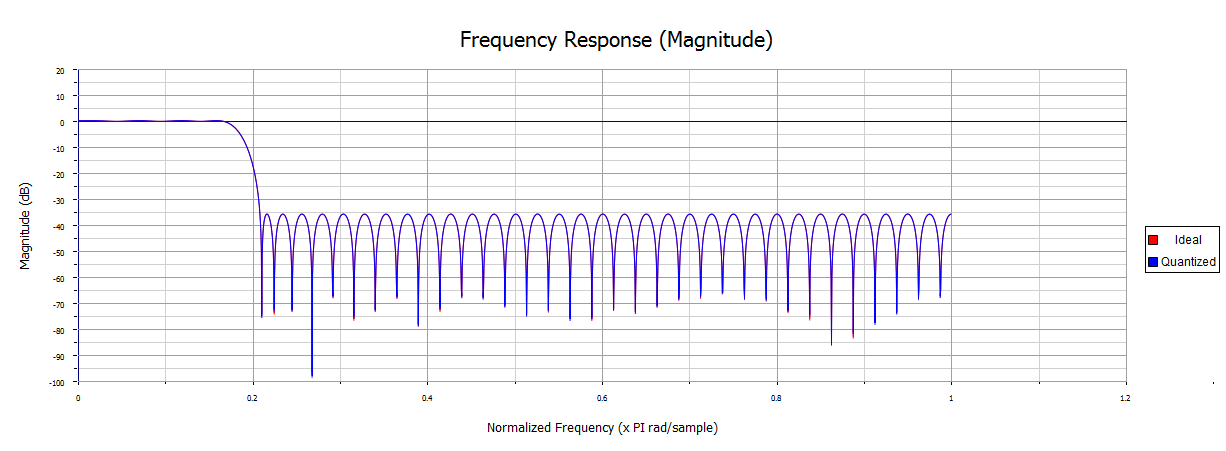
\includegraphics[scale=0.5]{LowPass_Filter_Design.png}
% 	\caption{A low pass filter design.}
% \end{figure}

%%%%%%%%%%%%%%%%%%%%%%%%%%%%%%%%%%%%%%%%%%%%%%%%%%%
%
%  New template code for TAMU Theses and Dissertations starting Fall 2016.
%
%
%  Original Author: Sean Zachary Roberson
%  This version adapted for URS by Parasol lab.
%  Adapted from version 3.16.10, which was last updated on 9/29/2016.
%  URS adaptation last updated 1/9/2017.
%
%%%%%%%%%%%%%%%%%%%%%%%%%%%%%%%%%%%%%%%%%%%%%%%%%%%
%%%%%%%%%%%%%%%%%%%%%%%%%%%%%%%%%%%%%%%%%%%%%%%%%%%%%%%%%%%%%%%%%%%%%%
%%                           SECTION IV
%%%%%%%%%%%%%%%%%%%%%%%%%%%%%%%%%%%%%%%%%%%%%%%%%%%%%%%%%%%%%%%%%%%%%

\chapter{CONCLUSION}

\section{Results}

Images of the application and textbook?

\section{Challenges}

Time? Tweaking existing build process of textbook for integration.

\section{Broader Impact}

Allow other authors to utilize this design + implementation?

\section{Future Plans}

Get this functional for entire MYMACalc book


%The next line is the format for inserting new sections.
%Replace the name "newsection"  with the name of your
%new section file.
%\include{data/newsection}


%fix spacing in bibliography, if any...
%%%%%%%%%%%%%%%%%%%%%%%%%%%%%%%%%%%%%%%%%%%%%%%%%%%%%%%%%%%%%
%\let\oldbibitem\bibitem
%\renewcommand{\bibitem}{\setlength{\itemsep}{0pt}\oldbibitem}
%%%%%%%%%%%%%%%%%%%%%%%%%%%%%%%%%%%%%%%%%%%%%%%%%%%%%%%%%%%%%%%
%The bibliography style declared is the IEEE format. If
%you require a different style, see the document
%bibstyles.pdf included in this package. This file,
%hosted by the University of Vienna, shows several
%bibliography styles and examples of in-text citation
%and a references page.

\phantomsection
\addcontentsline{toc}{chapter}{REFERENCES}

\renewcommand{\bibname}{{\large\rm\bf REFERENCES}}
%This file is a .bib database that contains the sources.
\bibliography{data/myReference}
\bibliographystyle{ieeetr}

%This next line includes appendices. The file
%appendix.tex contains commands pointing to
%the appendix files; be sure to change these
%pointers if you end up changing the filenames.
%Leave this commented if you will not need
%appendix material.

%%%%%%%%%%%%%%%%%%%%%%%%%%%%%%%%%%%%%%%%%%%%%%%%%%%
%
%  New template code for TAMU Theses and Dissertations starting Fall 2016.
%
%
%  Original Author: Sean Zachary Roberson
%  This version adapted for URS by Parasol lab.
%  Adapted from version 3.16.10, which was last updated on 9/29/2016.
%  URS adaptation last updated 1/9/2017.
%
%%%%%%%%%%%%%%%%%%%%%%%%%%%%%%%%%%%%%%%%%%%%%%%%%%%

% These are the commands to create an Appendix


%%%%%%%%%%%%%%%%%%%%%%%%%%%%%%%%%%%%%%%%%%%%%%%%%%%%%%%%%%%%%%%%%%%%%%
%%                           APPENDIX A
%%%%%%%%%%%%%%%%%%%%%%%%%%%%%%%%%%%%%%%%%%%%%%%%%%%%%%%%%%%%%%%%%%%%%

\phantomsection

\chapter*{First Appendix}
\addcontentsline{toc}{chapter}{\uppercase{First Appendix}}

Text for the Appendix follows.

\begin{figure}[h]
\centering
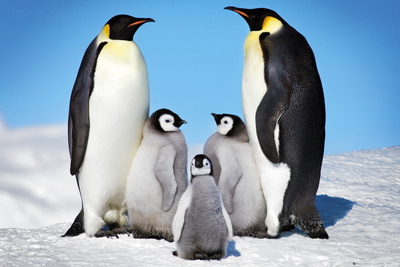
\includegraphics[scale=.50]{graphic/Penguins.jpg}
\caption{TAMU figure}
\label{fig:tamu-fig5}
\end{figure}

%%%%%%%%%%%%%%%%%%%%%%%%%%%%%%%%%%%%%%%%%%%%%%%%%%%%%%%%%%%%%%%%%%%%%%
%%                           APPENDIX B
%%%%%%%%%%%%%%%%%%%%%%%%%%%%%%%%%%%%%%%%%%%%%%%%%%%%%%%%%%%%%%%%%%%%%
\chapter*{A Second Appendix Whose Title Is Much Longer Than The First}
\addcontentsline{toc}{chapter}{\uppercase{A Second Appendix Whose Title Is Much
Longer Than The First}}

Text for the Appendix follows.

\begin{figure}[h]
\centering
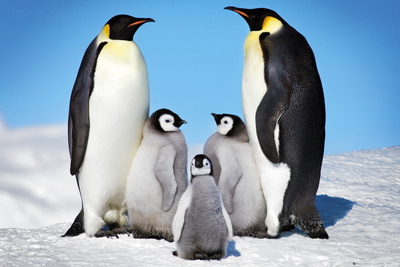
\includegraphics[scale=.50]{graphic/Penguins.jpg}
\caption{Another TAMU figure.}
\label{fig:tamu-fig6}
\end{figure}


\pagebreak{}



\end{document}
